Die    Aufgabe   eines    geschlossenen    Regelkreises (Abbildung \ref{fig:geschlossenerRegelkreis}) ist  es, einen  vorgegeben Sollwert  zu erreichen  und diesen
auch bei  St\"orungen aufrecht zu  erhalten. Dabei sollen die  unten genannten
dynamischen  Anforderungen  eingehalten  werden, damit  die  Stabilit\"at  des
Regelsystems garaniert ist. Die wichtigste  Bedingung f\"ur die Schrittantwort
ein  geschlossenen  Regelkreis heisst,  dass  der  Regelfehler, die  Differenz
zwischen Ist-und Sollwert, gleich Null oder m\"oglichst klein ist.\\


\begin{figure}[!h!, width=\pagewidth]
\begin{center}
    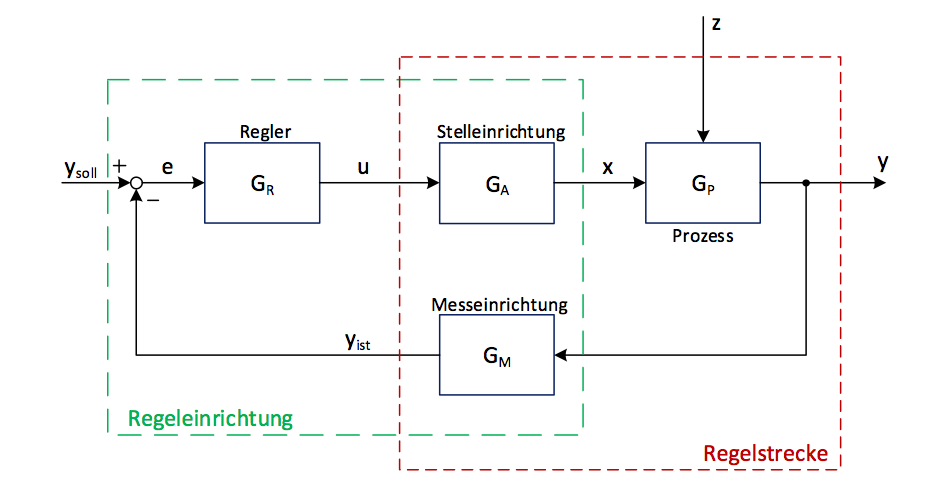
\includegraphics[width=0.5\textwidth]{images/geschlRegelkreis}
    \caption{Geschlossener Regelkreis}
    \label{fig:geschlossenerRegelkreis}
\end{center}
\end{figure}

%Name Bild Struktur eines allgemeinen Regelkreises
\begin{itemize}
    \item
        $y_soll$ bezeichnet den Sollwert der Regelgr\"osse.
    \item
        $e$ Regelabweichung (Regelfehler)
    \item
        $u$ Steuergr\"osse
    \item
        $x$ Stellgr\"osse
    \item
        $y$ Regelgr\"osse
    \item
        $z$ St\"orgr\"osse
    \item
        $y_ist$  ist der  Ist-Wert der  Regelgr\"osse  und wird  auch als  die
        Schrittantwort des Regelkreis bezeichnet.
\end{itemize}

\todo{Bild Schrittantworten passend zu Aufzählung unten}

Grunds\"atzlich  k\"onnen  f\"unf   Anforderungen  f\"ur  einen  geschlossenen
Regelkreis und deren Schrittantworten zusammengefasst werden:\\
\begin{enumerate}
    \item Der Regelkreis muss stabil sein:
        \begin{itemize}
            \item
                Das heisst  f\"ur die Schrittantwort, dass  nach dem Erreichen
                des  eingeschwungenen  Zustand kein  erneutes  \"Uberschwingen
                stattfinden darf.
            \item
                F\"ur  das  Regelsystem  heisst  stabil,  dass  es  in  seinen
                Gleichgewichtszustand zur\"uckgef\"uhrt werden kann.
        \end{itemize}
    \item
        Der Regelkreis  muss gen\"ugend ged\"ampft sein: \\Die  D\"ampfung der
        Schrittantwort soll  so stark  sein, dass der  eingeschwungene Zustand
        m\"oglichst  rasch erreicht  wird  ohne dass  das \"Uberschwingen  des
        Systems zu stark wird.
    \item
        Der   Regelkreis   muss   eine  bestimmte   station\"are   Genauigkeit
        aufweisen: Das  bedeutet,  der  Regelfehler  e(t) soll  f\"ur  t->  oo
        gegen  Null  gehen. F\"ur  die  Schrittantwort heisst  das,  dass  die
        Schrittantwort gleich $y_soll$ sein muss.
    \item
        Der Regelkreis  muss hinreichend  schnell sein: Die  Schnelligkeit des
        Einschwingvorganges der  Schrittantwort ist  stark von  der D\"ampfung
        abh\"angig. Ist die D\"ampfung  zu stark oder zu  schwach, braucht der
        Einschwingvorgang mehr Zeit. Hierbei muss darauf geachtet werden, dass
        die spezifischen Anforderungen an das Regelsystem eingehalten werden.
    \item
        Der  Regelkreis muss  robust  sein: Der Regelkreis  muss so  ausgelegt
        werden,  dass  das  Regelsystem  auch im  schlimmsten  Fall  (je  nach
        Regelsystem situationsabh\"angig) in der Lage ist, das System zur\"uck
        in den stabilen Zustand (vgl. 1.) zu regeln.
\end{enumerate}
